\documentclass[11pt,a4paper]{article}
\usepackage{ls}
\usepackage[ngerman]{babel}

\title{Zur Methodik des TRIZ-Trainers und AIPS-2015}

\author{Hans-Gert Gr\"abe, Leipzig}

\date{14. Juli 2020, Update 9. Oktober 2020}

\begin{document}
\maketitle
%\tableofcontents

\subsection*{TRIZ und die Welt der Widersprüche}

In der TRIZ-Welt geht es um Widersprüche in der Arbeitsweise zu entwerfender
oder real existierender technischer Systeme. Technische Systeme sind dabei
stets in der Einheit von Beschreibungs- und Vollzugsform zu verstehen, wobei
diese Einheit im Sinne von \cite{Graebe2020} dialektischer Natur ist -- in der
Beschreibungsform spielt Einheit in der Vielfal die zentrale Rolle, in der
Vollzugsform die Rückgewinnung von Vielfalt aus der Einheit.  Diese abstrakte
Formulierung ist wie folgt zu verstehen: Aus der Vielfalt werden abstrakte
\emph{technische Prinzipien}\footnote{Dieser Begriff „Prinzip“ ist nicht mit
  demselben Wort in der Konnotation als „TRIZ-Prinzip“ identisch, der eine
  unglückliche Übersetzung des russischen Worts „Prijom“ ist, das besser als
  „Vorgehensweise“ übersetzt wäre.} abgehoben und technikwissenschaftlich zu
\emph{Verfahren} verdichtet. In der Vollzugsform kommen dagegen \emph{mehrere}
solche Verfahren im Zusammenspiel zum Einsatz, um ein konkretes technisches
Problem zu lösen. Dies wird allerdings ebenfalls von einer Beschreibungsform
begleitet, einer \emph{Beschreibungsform 2. Art}, die von den gerade
eingeführten Beschreibungsformen 1. Art für domänenspezifische technische
Prinzipien zu unterscheiden ist und das \emph{Zusammenspiel} der Prinzipien in
der konkreten technischen Lösung zum Gegenstand hat.

Diese Unterscheidung zieht sich durch bis in die Berufsbilder -- konkrete
technische Verfahren werden von Spezialisten entwickelt, konkrete technische
Lösungen von Generalisten, siehe dazu ausführlich \cite[Abschnitt
  9]{Graebe2020}.   Allerdings ist die Welt nicht so dichotom aufgebaut,
sondern eher fraktal.  Spezialisten in einer Perspektive können durchaus
Generalisten in einer anderen Perspektive sein, wenn es nämlich um ein
spezielles Domänenproblem geht, zu dessen Lösung Spezialisten aus anderen
Domänen herangezogen werden müssen.

\subsection*{TRIZ als Methodik für Generalisten}

TRIZ ist in diesem Sinne eine Methodik für Generalisten, die zu Einzelfragen
Spezialisten hinzuziehen. Dieser für erfolgreiche praktische Anwendungen der
Methodik sehr wichtige Team-Player-Ansatz ist in der TRIZ-Methodik kaum
ausgearbeitet.  Im Gegenteil, die Methodik geht von der zentralen Rolle einer
„schöpferischen Persönlichkeit“ aus und sieht diese in einer bedeutenden
verfahrensleitenden Position. Konfliktäre Situationen mit dem Management
werden dabei eher unter privat-psychologischen und weniger unter strukturellen
Gesichtspunkten abgehandelt.

In der TRIZ-Ausbildung geht es darum, diesen Generalisten in seiner Arbeit
methodisch zu unterstützen. In der \emph{fortgeschrittenen TRIZ-Ausbildung}
geht es darum, komplexe Anforderungssituationen mit einer größeren Zahl sowohl
von Komponenten als auch von Widersprüchen zu modellieren und zu analysieren,
wobei SF-Modellierung, RCA, CECA und Entwicklungstrends technischer Systeme
als Instrumente im Vordergrund stehen, um sich in einer komplexen
Widerspruchslandschaft zurechtzufinden und überhaupt erst einen Ansatzpunkt
für ein Problem zu finden, an dem die in der \emph{TRIZ-Grundausbildung}
erworbenen Fertigkeiten der Problemanalyse angewendet werden können.

Beiden Ausbildungsformen gemeinsam ist das Bild einer vorgefundenen Welt stark
interdependenter technischer Systeme. Ein solches Bild geht von Beschreibungs-
und Vollzugsformen der \emph{unmittelbaren} Interaktion zwischen diesen
Systemen aus und blendet höhere Formen der Abstraktion wie Frameworkmodelle
dieser Interaktionen weitgehend aus, da die TRIZ-Methodik selbst eine
Interaktionsabstraktion auf dieser Analyseebene ist.  Siehe
\cite{Szyperski2002} für grundsätzliche Überlegungen zu derartigen höheren
Formen der Abstraktion von „Wiederverwendeung“.

Ein solches spezifisches Bild eines Generalisten von der Welt der technischen
Systeme wird im Weiteren als konstitutiv für die TRIZ-Methodik vorausgesetzt.
Im ersten Zugriff sind dabei technische Systeme abgrenzbare \emph{Black
  Boxes}, die in der Beschreibungsform durch ihre \emph{Spezifikation} und in
der Vollzugform durch \emph{spezifikationskonformes Verhalten} charakterisiert
sind.  Die Interaktionen zwischen den Systemen sind in der Beschreibungsform
als \emph{Zwecke} gegeben, in der Vollzugsform als \emph{Flüsse}, die sich für
die einzelnen Systeme als für deren Funktionieren wesentliche
\emph{Durchsätze} manifestieren.

\begin{figure}
  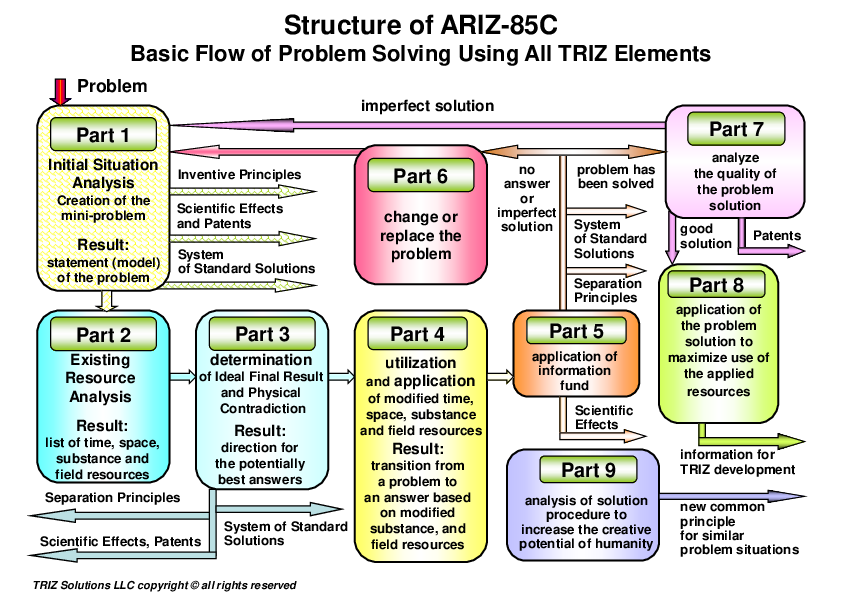
\includegraphics[width=.9\textwidth]{ARIZ-Workflow.png}
  \caption{Der ARIZ-85C Workflow in schematischer Darstellung nach I. Bukhman}
\end{figure}


In der TRIZ-Grundausbildung geht es darum, widersprüchliches Verhalten durch
genauere Analyse \emph{eines} kritischen Systems abzustellen, ohne dass
methodisch klar werden muss, \emph{wie} dieses kritische System überhaupt
identifiziert wird.  Genau so geht ARIZ-85C vor: Am Ende („no answer or
imperfect solution“) heißt es „Part 6: change or replace the problem. Back to
Part 1“. Die \emph{Auswahl} des genauer zu analysierenden kritischen Systems
erfolgt also weitgehend heuristisch und ist zusammen mit einer ersten Analyse
des inneren Funktionierens dieses Systems als \emph{White Box} Gegenstand der
ersten Phase des TRIZ-Trainers.  Dies entspricht im Wesentlichen Teil 1 von
ARIZ-85C.  Davon zu unterscheiden ist das Vorgehen sowohl in der
TRIZ-Fortgeschrittenenausbildung (etwa PICC \cite{Cavallucci} von
D. Cavallucci und dessen IDM-Ansatz) als auch das Vorgehen in komplexeren
industriellen Anwendungssituationen, wo für diese Analyse weitere
TRIZ-Instrumente eingesetzt werden.

\subsection*{Das System und seine Nachbarsysteme}

In einer \emph{Welt der technischen Systeme} gibt es keine Obersysteme. Die
herausgehobene Rolle der Obersystem-System-Beziehung in der TRIZ-Methodik
wurde bereits in \cite[S. 16]{Graebe2020} kritisiert und festgestellt, dass
diese Beziehung von ihren Charakteristika her mehr oder weniger identisch ist
mit der System-Komponenten-Beziehung. Ich komme darauf weiter unten zurück.
In einer Welt der Systeme sind für ein zu untersuchendes System vor allem
diejenigen Nachbarsysteme wesentlich, zu denen eine enge kausale Beziehung
besteht.  Es ist zu erwarten, besonders nach Phasen des \emph{Trimmens}, dass
\emph{mehrere} solche Nachbarsysteme kausal wichtig sind.  Für Anwendungen im
TRIZ-Trainer wollen wir allerdings annehmen, dass es nur \emph{ein} solches
wesentliches Nachbarsystem gibt, das Quelle von Zweck (Beschreibungsform) und
ggf. Durchsatz (Vollzugsform) für das zu untersuchende System ist. Dieses
Nachbarsystem wollen wir dann doch wieder als \emph{Obersystem} bezeichnen.

\subsection*{TRIZ-Trainer -- die erste Phase des Lösungsprozesses}

Im Minsker TRIZ-Trainer kommt die algorithmische Version
AIPS-2015\footnote{AIPS ist ein russisches Akronym und steht für „Algorithmus
  der Veränderung problematischer Situationen“.} der TRIZ-Theorie zum Einsatz,
die unter \cite{TRIZTrainer.Problemloesungsprozess} genauer beschrieben ist.
Die Kenntnis dieser Ausführungen wird im Weiteren vorausgesetzt.

Für den ersten Abschnitt „Präzisierung der Umstände“ der ersten Phase „Analyse
der Problemsituation“ im TRIZ-Trainer ergibt sich damit folgende
Aufgabenstellung:
\begin{itemize}
\item [1.] Identifiziere das zu untersuchende System als Black Box und gib ihm
  einen „sprechenden Namen“, aus dem sich die Semantik des Systems bereits
  grob erschließt -- statt „nützliches Produkt“. 
\item [2.] Identifiziere das Obersystem (sprechender Name) sowie Zweck
  (Bedeutung des Systems für das Obersystem) und ggf. Durchsatz (Leistung des
  Obersystems für das Funktionieren des Systems) -- „nützliches Prinzip“ (des
  Systems). 
\item [3.] Formuliere das bestehende Problem, welches spezifikationskonformem
  Verhalten des Systems im Wege steht -- „unerwünschter Effekt“.
\end{itemize}
Daran schließt als zweiter Abschnitt „Systemkonflikt“ die genaue Modellierung
des Systems als White Box sowie die Identifizierung der Konfliktstruktur an.
Das als White Box zu untersuchende System wird dabei verallgemeinernd als
\emph{Maschine} bezeichnet, siehe dazu auch die Ausführungen im
Online-Hilfesystem des TRIT-Trainers.

Für diesen zweiten Abschnitt ergibt sich damit folgende Aufgabenstellung:
\begin{itemize}
\item [4.] Bestimme die Bestandteile der Maschine (deren Aufbauorganisation)
  -- „Maschine“ sowie deren Arbeitsweise (deren Ablauforganisation) -- „Wie
  die Maschine arbeitet“. Oft reicht es aus, den Schwerpunkt auf eine der
  beiden Fragen zu legen.

  Dabei ist das im Online-Hilfesystem genauer erläuterte allgemeine
  Aufbaumuster „Energiequelle, Antrieb, Transmission, Werkzeug, Aktion,
  bearbeitetes Objekt, nützliches Produkt plus Steuerung“ auf die konkrete
  Modellierungssituation herunterzubrechen.
  
  Hierbei ist es wichtig, nicht nur das Problem selbst im Auge zu haben,
  sondern auch die primär nützliche Funktion (PNF) des Systems zu beschreiben.
  Um diese herum gruppieren sich die im System genutzten Ressourcen, so dass
  sich aus dieser Perspektive später ein besonders genaues Bild ergibt, welche
  Ressourcen zur Lösung des Problems besonders leicht zugänglich sind. 

\item [5.] Diese PNF steht in gewissem Verhältnis zur „Wirkung, die nicht ohne
  Probleme abgeschlossen werden kann“. Diese Wirkung sowie ihr Verhältnis zur
  PNF sind nun genauer zu bestimmen. Dieses Verhältnis ist der Kern des zu
  lösenden Konflikts.  Bei dieser Analyse sind insbesondere Ort und Zeit des
  Konflikts genauer einzugrenzen, um mögliche spätere Separationen nach Ort
  oder Zeit als grundlegende Lösungsmethoden vorzubereiten. 
\end{itemize}

Im dritten Abschnitt „Aufstellen einer Hypothese“ sind durch genauere Analyse
der „Konflikt"|ursachen“ eine oder (gern auch) mehrere Hypothesen allgemeinen
Charakters aufzustellen, welche Maßnahmen im Sinne eines \emph{idealen
  Endresultats}\footnote{Das \emph{Ideale Endresultat} ist einer der
  TRIZ-Grundbegriffe. Mit ihm wird beschrieben, wie die Lösung (Maschine)
  beschaffen sein müsste, die alle unsere im Aufgabenkontext formulierten
  Wünsche erfüllt, ohne dass wir bereits wissen, ob und wie diese Maschine
  gebaut werden kann.  Das IER ist eine Orientierungsgröße im Sinne einer
  „konkreten Utopie“, die wesentlich den Zielkorridor bestimmt, auf den sich
  der weitere Lösungsprozess in der zweiten Phase konzentriert.} das Problem
lösen würden.  Einer dieser Ansätze wird als „Bedingungen der Aufgabe“ genauer
formuliert, um diese dann in der zweiten Phase des Lösungsprozesses mit den
TRIZ-Werkzeugen zu bearbeiten.

\subsection*{Nachbarsysteme und Komponenten}

Bei der Modellierung des zu untersuchenden Systems als White Box ist zu
beachten, dass es selbst Leistungen aus anderen Systemen über deren
Schnittstellen bezieht. Typischerweise sind das Komponenten des Systems, die
innerhalb der Systemmodellierung als Black Boxes betrachtet werden, deren
Leistungsfähigkeit über eine Schnittstellenspezifikation beschrieben wird und
deren praktische Leistung durch spezifikationskonformes Verhalten einen
\emph{Durchsatz} durch das System erzeugt, der für das Funktionieren des
Systems konstitutiv ist. Der \emph{äußere} Durchsatz, welcher das System am
Leben erhält, kommt also zu einem Teil aus dem \emph{Inneren} des Systems.
Bei der Suche nach Ressourcen mit gewissen Eigenschaften, etwa als
X-Komponente, kann es darüber hinaus sein, dass externe Ressourcen
nachträglich in die Systemmodellierung integriert werden (im Sinne des
TRIZ-Trends 2 „increasing system completeness“). In einer Welt technischer
Systeme können dies aber nur Nachbarsysteme sein, so dass im Zuge der
Systemmodellierung (allerdings erst in der zweiten Phase „Lösung der Aufgabe“
im TRIZ-Trainer) ein natürlicher Prozess der Transformation von
Nachbarsystemen in Systemkomponenten zu berücksichtigen ist. Hier kann die
strukturelle Verhältnisähnlichkeit (in der Modellierung des Systems erscheinen
die Nachbarsysteme in gleicher Weise als Black Boxes wie die Komponenten und
sind wie diese auch nur über Schnittstellenspezifikationen ansprechbar) zur
Verschmelzung von zwei Begriff"|lichkeiten -- Komponente und Nachbarsystem --
\emph{im Rahmen des spezifischen Modellierungskontextes} weitergetrieben
werden. Da sich andererseits die Modellierung der Interna des zu
untersuchenden Systems in der zweiten Etappe „Systemkonflikt“ der ersten Phase
im TRIZ-Trainer sowieso auf \emph{Wesentliches} (wesentliche Komponenten und
wesentliche Beziehungen) nach vorgegebenem methodischem Muster (Energiequelle,
Transmission, Werkzeug, ..., Steuerung) reduziert, besteht kein Problem,
zunächst \emph{alle} Nachbarsysteme als Komponenten in die Modellierung des zu
untersuchenden Systems und die Beziehungen zwischen ihnen als Beziehungen
zwischen Komponenten aufzunehmen.

Dies ist freilich ein formaler, für den TRIZ-Neuling weitgehend transparenter
Schritt, der von der Selektion der für die innere Logik des Systems
\emph{wesentlichen} Komponenten und Beziehungen im APIS-2015 nicht separiert
ist und nicht separiert werden soll.  Der methodische Vorteil ist allerdings,
dass das zu modellierende System \emph{in diesem Modellierungskontext} dann
kein Außen mehr hat.

Im APIS-2015 wird für die Suche nach Ressourcen ein Schalenmodell
vorgeschlagen (Hilfesystem \emph{Lösungsprozess $\to$ Suche nach einer
  Ressource}), nach dem in die Suche Schritt für Schritt
\begin{enumerate}[noitemsep]
\item die operative Zone mit Werkzeug und verarbeitetem Objekt,
\item Systemkomponenten im Umfeld der operativen Zone,
\item Systemkomponenten überhaupt (d.h. solche, die in der vorausgegangenen
  Modellierung bereits als Teil des Systems identifiziert wurden),
\item leicht verfügbare Ressourcen aus der Umgebung (dem „Obersystem“),
\item Maschinenkomponenten (das ist in gewissem Sinne redundant) und
\item Umweltkomponenten
\end{enumerate}
einbezogen werden. Eine Unterscheidung zwischen Ressourcen und Komponenten
bleibt in der Betrachtung vage, Ressourcen sind der allgemeinere Begriff und
umfassen auch „natürliche“ Ressourcen, obwohl zu jeder für den Einsatz im
System nützlichen Ressource auch eine (und sei es rudimentäre)
\emph{Beschreibung} ihrer „nützlichen“ Eigenschaften im Form eines
Black-Box-Modells vorliegen muss. Insoweit unterscheiden sich die Begriffe nur
graduell. 

Für die Suche nach Ressourcen ist eine gute Funktionsanalyse \cite[Abschnitt
  4.4]{Koltze2017} wichtig, um die geforderten Eigenschaften der Ressource
möglichst genau zu beschreiben.  In fortgeschrittenen Anwendungen ist auch das
Gegenteil hilfreich, nämlich die genaue Kenntnis der Eigenschaften von
Ressourcen in einer \emph{Effektendatenbank} wie in \cite[Abschnitt
  8.2]{Koltze2017} genauer beschrieben sowie das Potenzial einer
\emph{funktionsorientierten Suche} wie in \cite[Abschnitt 4.14]{Koltze2017}
genauer beschrieben, die gezielt nach genauer spezifizierten Funktionalitäten
gleicher Bauart in anderen Technikbereichen sucht. 
\newpage
\bibliographystyle{plain}
\begin{thebibliography}{xxx}
\bibitem{Cavallucci} Denis Cavallucci. PICC Solutions. Augmented Human
  Intelligence.  \url{https://www.picc-solution.com/}
\bibitem{Graebe2020} Hans-Gert Gräbe (2020). Die Menschen und ihre Technischen
  Systeme. LIFIS Online, Mai 2020. \url{doi:10.14625/graebe_20200519}
\bibitem{Koltze2017} Karl Koltze, Valeri Souchkov (2017). Systematische
  Innovationsmethoden. Hanser, München. 
\bibitem{Szyperski2002} Clemens Szyperski (2002). Component Software. Addison
  Wesley, Boston. 
\bibitem{TRIZTrainer.Problemloesungsprozess} TRIZ-Trainer.
  Problemlösungsprozess.  Beschreibung des Lösungsprozesses nach dem
  AIPS-2015-Algorithmus.  \url{https://triztrainer.ru/process-resheniya/}
\end{thebibliography}

\end{document}
